\section{Case Study: Closed-loop Model Checking of a Dual Chamber Pacemaker}
\label{caseStudy}
\begin{figure}[!t]
	\centering
	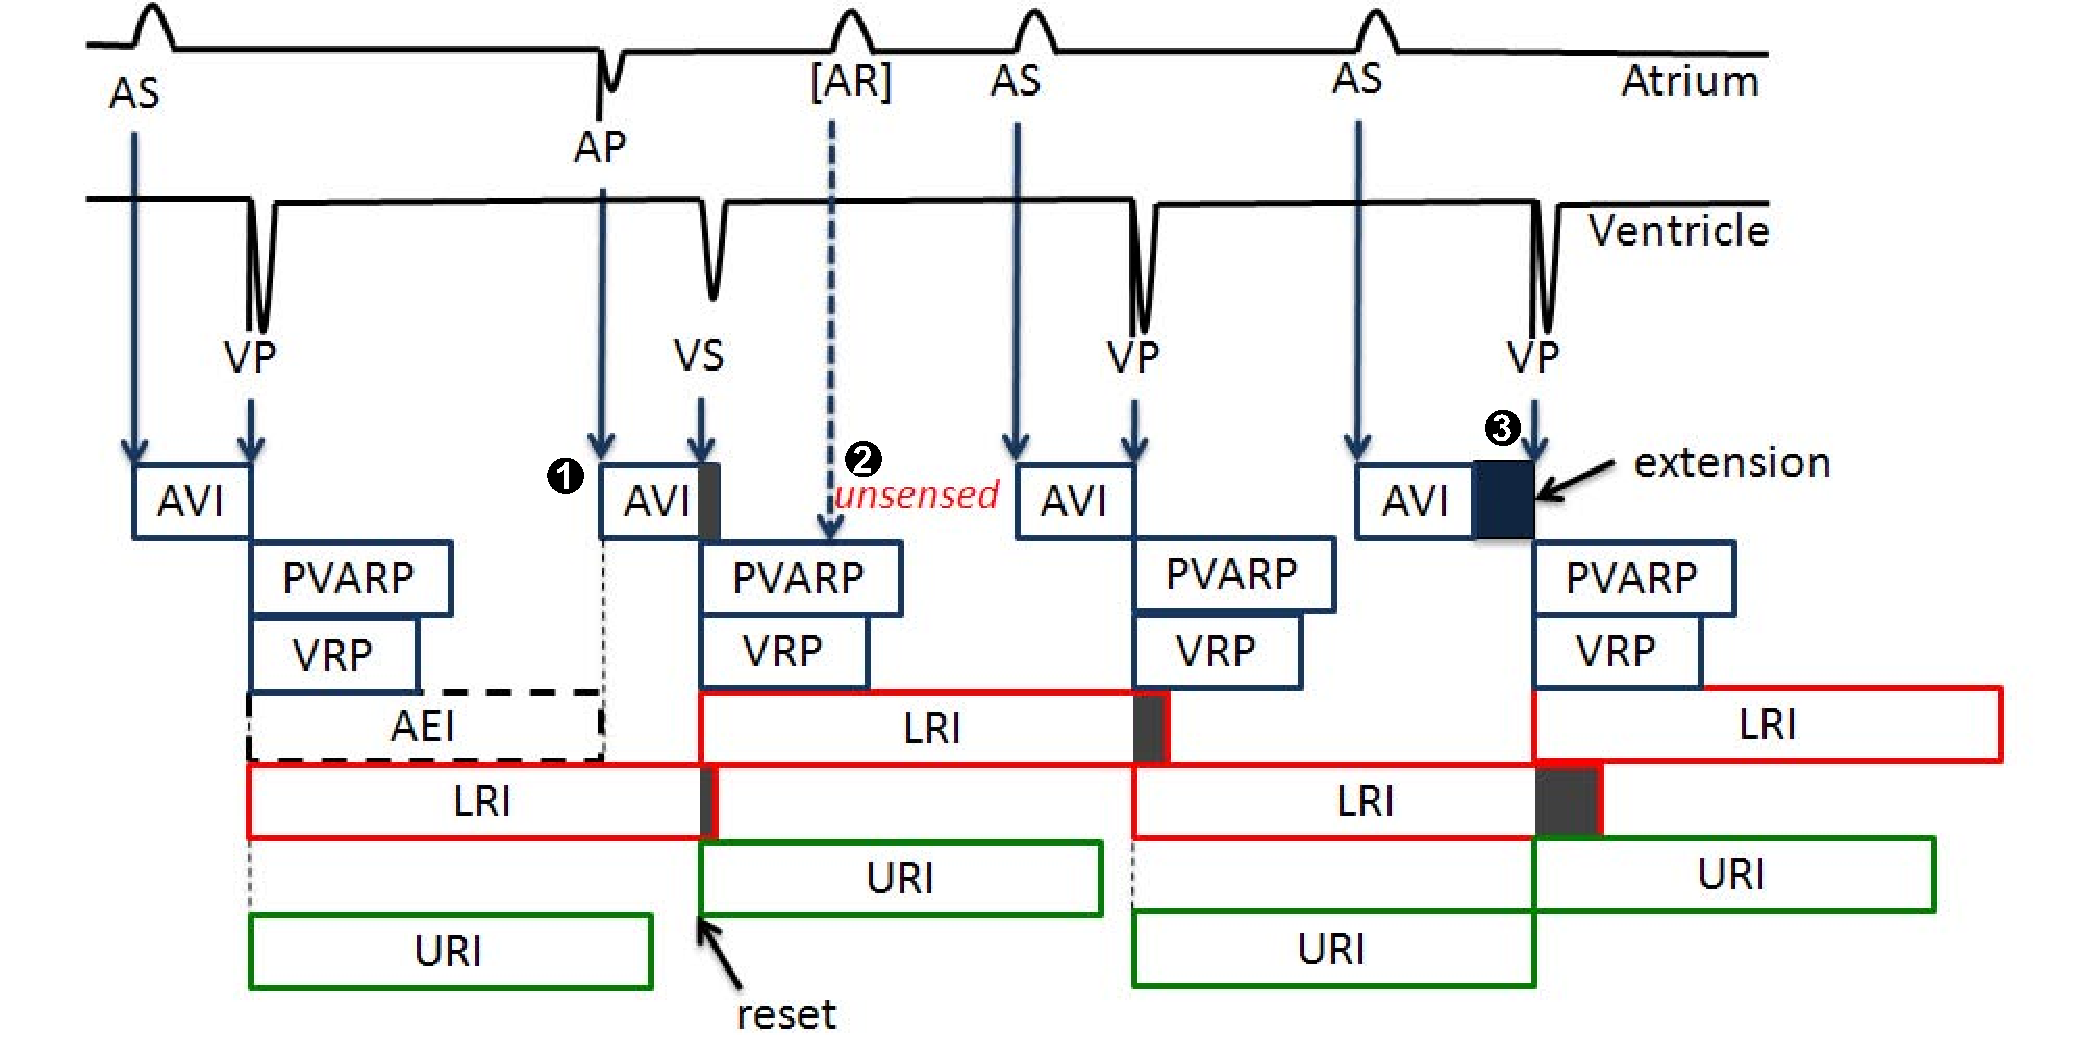
\includegraphics[width=0.8\textwidth]{figs/PM_timers.pdf}
	%\vspace{-5pt}
	\caption{\small Basic timers for a dual chamber pacemaker. AS: Atrial Sense, VS: Ventricular Sense, AP: Atrial Pacing, VP: Ventricular Pacing.}
	%\vspace{-15pt}
	\label{fig:PM_timers}
\end{figure}

\subsection{Pacemaker Model}
A pacemaker diagnoses heart conditions and deliver electrical pacing to the heart according to the timing intervals among timing events from the heart and the pacemaker itself. In this section we use a simple dual chamber pacemaker as example for closed-loop model checking. The detailed UPPAAL timed automata implementation of the model can be found in \cite{sttt13}. A dual chamber pacemaker has several basic timers, which are shown in \figref{PM_timers}:\\
\textbf{Atrial Escape Interval (AEI)} defines the maximum interval between the last ventricular event (VS,VP) to an atrial event (AS,AP). If no AS happened before AEI timer runs out, atrial pacing (AP) is delivered to the heart (Marker 1 in \figref{PM_timers}). \\
\textbf{Atrio-Ventricular Interval (AVI)} defines the maximum interval between the last atrial event (AS,AP) to an ventricular event (VS,VP). If no VS happened before AVI timer runs out, and the time since the last ventricular event (VS,VP) is no less than URI, ventricular pacing (VP) is delivered to the heart (Marker 3 in \figref{PM_timers}).\\
\textbf{Post-Ventricular Atrial Refractory Period (PVARP) and Ventricular Refractory Period (VRP)} define the minimum period that a AS or VS can happen since the last ventricular event (VS,VP). 

\subsection{Requirement Encoding}
The requirement below is designed to prevent the pacemaker from pacing too fast.\\
\textsf{If intervals between self-activations of the atria is between 300ms to 1000ms, the intervals between ventricular paces should be no shorter than 500ms.}

With parameter mapping and a monitor $M_{sing}(VP,500,\infty)$, the requirement can be translated to:
$$Req1: N_A.loc=Rest \&\& N_A.t\in [300,1000] \Rightarrow \neg M_{sing}.Err$$
\begin{figure}[!b]
	\centering
	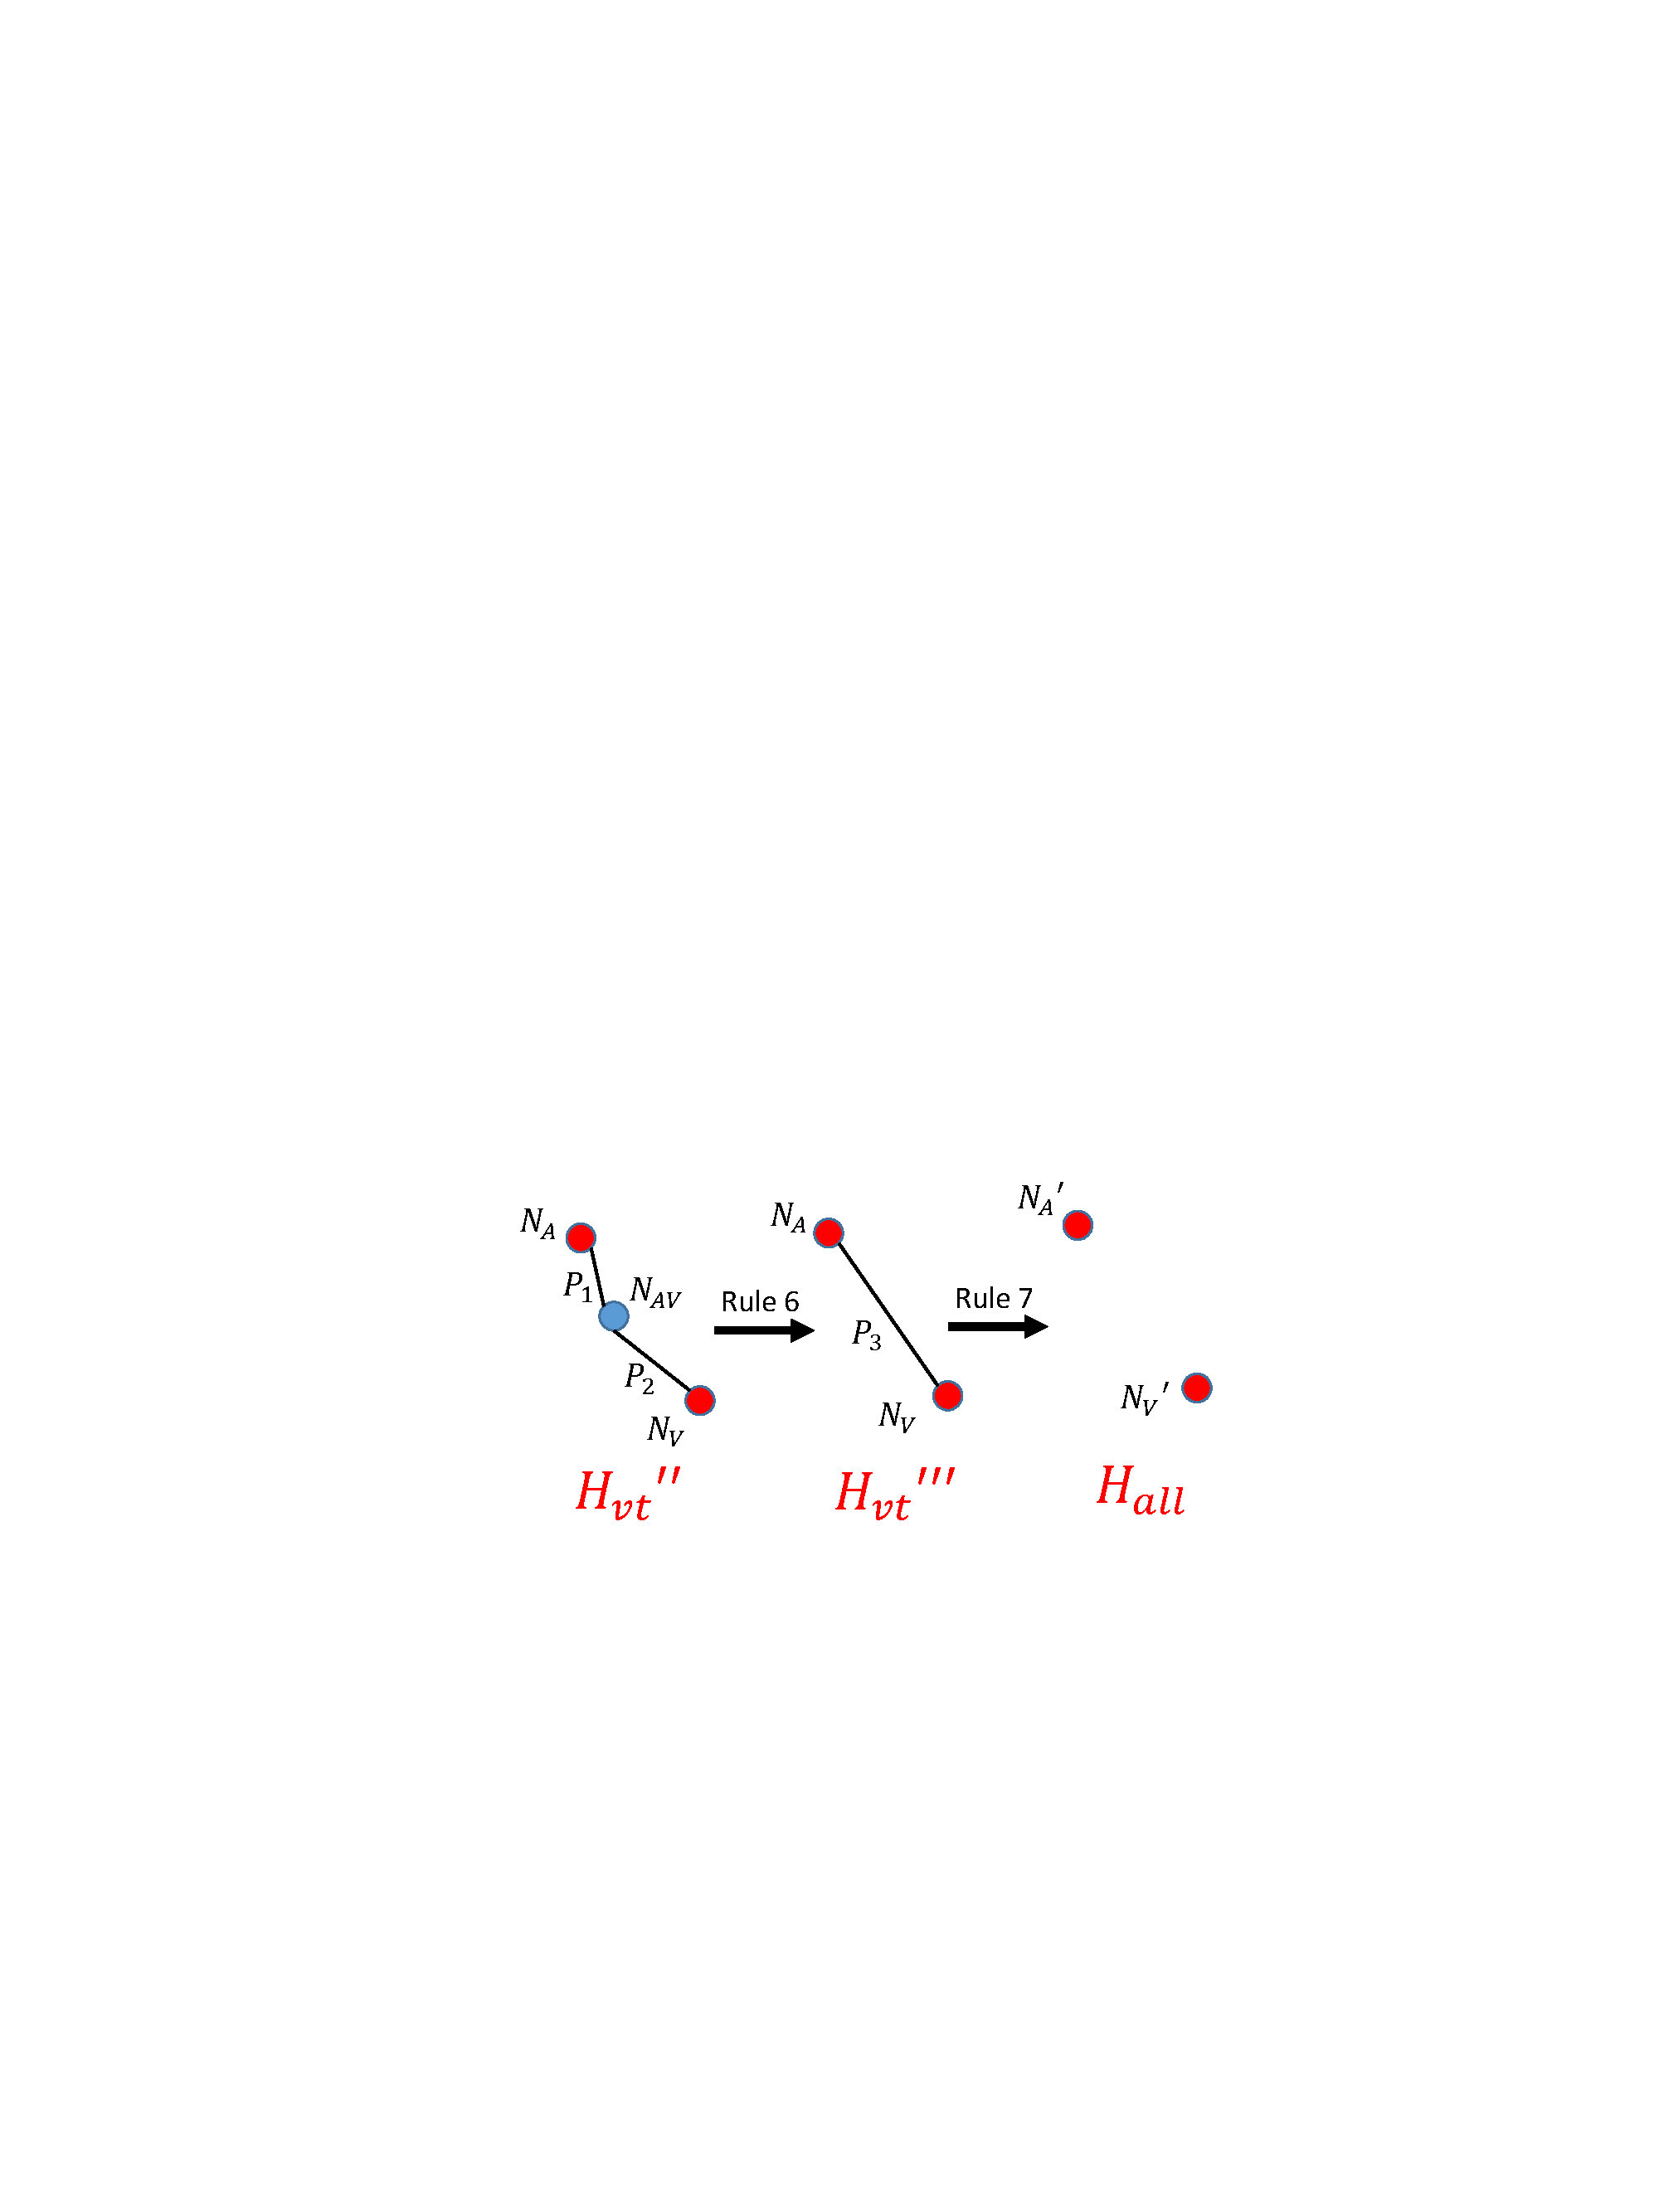
\includegraphics[width=0.5\textwidth]{figs/abs_sim.pdf}
	%\vspace{-5pt}
	\caption{\small Abstraction Rule Application Example}
	%\vspace{-15pt}
	\label{fig:abs_exam}
\end{figure}
 \subsection{Choosing Appropriate Heart Model For the Requirement}
To verify the closed-loop system with pacemaker model $PM$ and heart model abstraction tree $HM\_tree$ (\figref{HM_abs}) against requirement $Req1$, we start by searching for the most abstract appropriate models from the abstraction tree. We call the function specified in Algorithm 1: $[HM]=eligible(HM\_tree,Req1)$. The variables in the requirement and the corresponding monitor are:
$$Var(Req1)\cup Var(M_{sing})=\{N_A.t,N_A.loc, VP\}$$

At the root level heart model $H_{all}$, we have $\{N_A.t,N_A.loc\}\not\in Var(H_{all})$. As the result, $H_{all}$ is not appropriate for $Req1$. For all the children of $H_{all}$: $H_n'',H_{at}'''',H_{vt}'''$, we have $Var(Req1)\cup Var(M_{sing})\subseteq Var(H_n'')=Var(H_{at}'''')=Var(H_{vt}''')$, thus these 3 heart models are outputted as the most abstract models that are appropriate for $Req1$.

\subsection{Providing Unambiguous Counter-examples to the Physicians}
After we choose the appropriate models for $Req1$, we have: 
$$HM=\{H_n'',H_{at}'''',H_{vt}'''\}$$
Then we run Algorithm 2. By model checking on all 3 initial models in UPPAAL we have: 
$$[1,[]]=ModelChecking(H_n'',PM,Req1)$$
 $$[0,CE_1]=ModelChecking(H_{at}'''',PM,Req1)$$
$$[0,CE_2]=ModelChecking(H_{vt}''',PM,Req1)$$
For the two heart models $H_{at}'''',H_{vt}'''$ in which the requirement is violated, the algorithm keeps going down the abstraction tree, and upon termination counter-examples are returned for the following heart models:
$$H_{at};H_{pvc};H_{af};H_{avn};H_{afib}$$
%$$[0,CE_{at}]=ModelChecking(H_{at},PM,Req1)$$
%$$[0,CE_{pvc}]=ModelChecking(H_{pvc},PM,Req1)$$
%$$[0,CE_{af}]=ModelChecking(H_{af},PM,Req1)$$
%$$[0,CE_{avn}]=ModelChecking(H_{avn},PM,Req1)$$
%$$[0,CE_{afib}]=ModelChecking(H_{afib},PM,Req1)$$

\begin{figure}[!t]
		\centering
		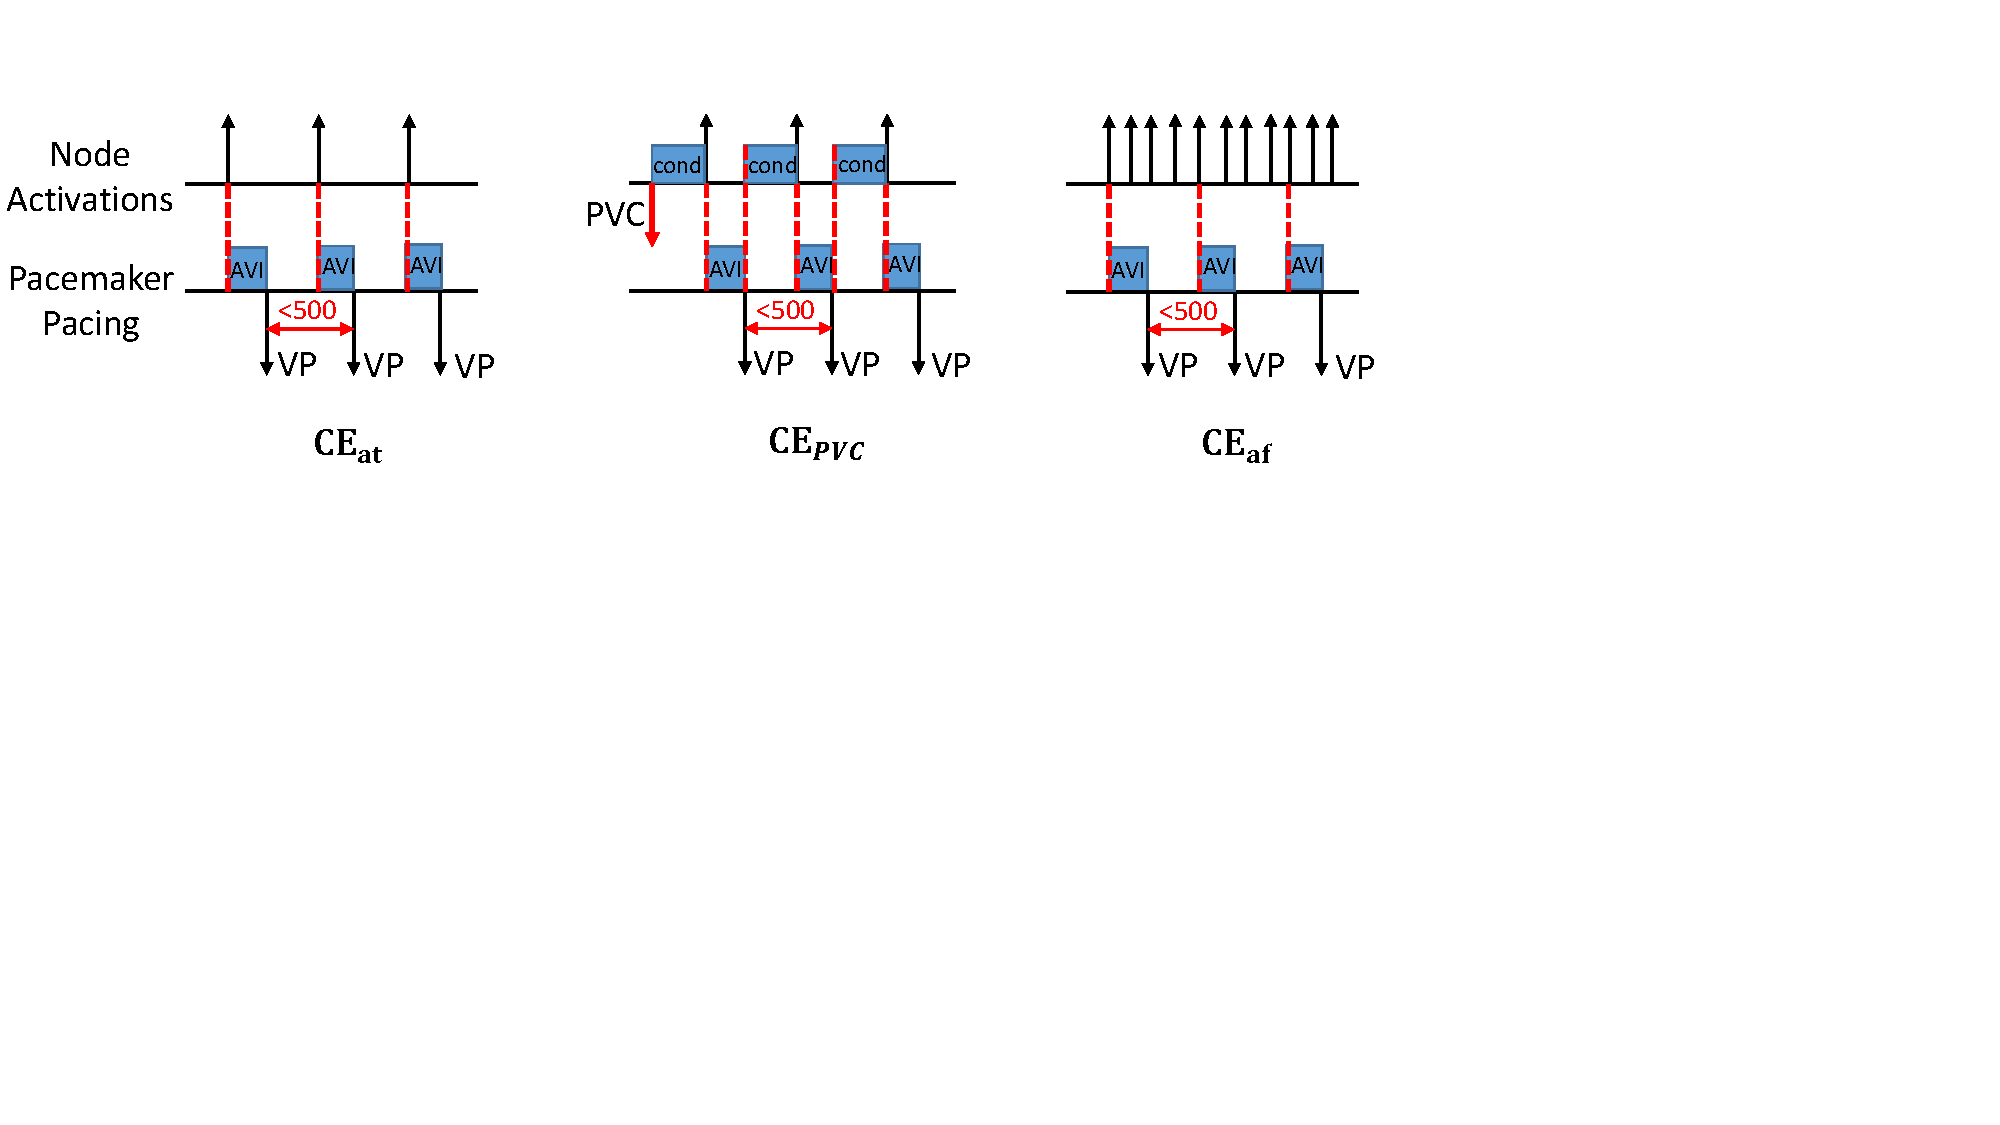
\includegraphics[width=0.9\textwidth]{figs/case.pdf}
		%\vspace{-5pt}
		\caption{\small Counter-examples}
		  %\vspace{-15pt}
		\label{fig:CE}
\end{figure}

The counter-examples are then sent to physicians for analysis. In \figref{CE} we demonstrate 3 counter-examples from the case study. We only show the activations of the atrial node and ventricle pacing. 
$CE_{at}$ corresponds to fast intrinsic heart rate (i.e. when running). The pacemaker is pacing the ventricle after $TAVI$ period to maintain optimal A-V delay, which is a safe execution. 

$CE_{pvc}$ has a very similar execution with $CE_{at}$. However, the activations of the atrial node is triggered by retrograde conduction from ventricular paces (marker \textsf{cond}). The atrial activations trigger another ventricular pace after $TAVI$, which will trigger another retrograde conduction. In this case the heart rate is controlled by $TAVI+Tcond$, which corresponds to an inappropriate closed-loop behavior called Endless Loop Tachycardia.

In $CE_{af}$ the atrial rate is very high, which is a sub-optimal heart condition. However, the ventricular rate can stay normal due to the blocking property of the AV node. Despite the filters in the pacemaker, the pacemaker still paces the ventricle for every 3 atrial activations, which extends fast atrial rate to more dangerous fast ventricular rate. This scenario is referred to as Atrial Tachycardia Response of a pacemaker. 

From the analysis, pacemaker operations in $CE_{pvc}$ and $CE_{af}$ need to be revised. However, the revision should not affect the behavior in $CE_{at}$. This example demonstrates that counter-examples from more refined models provide more detailed mechanism of the requirement violations, and distinguish the physiological conditions that can trigger the violations. The information is helpful for debugging and improving the algorithm. The physicians can also improve the physiological requirement so that these heart conditions can be then considered case by case. %Both $CE_b$ and $CE_c$ are inappropriate executions of the pacemaker .$CE_a$ and $CE_b$ can have the same input-output executions on the pacemaker side and can only be differentiated on the heart model side. After the physician examines the counter-example the programmer can work on debugging. 
%$NA\_self$ is in $H_3$, we go one level up, in $H_4$ the behavior is not merged with any other parameters. In $H_5$ $NA\_self$ is merged with  $NA'-NV'.cond$ so $H_4$ is returned as the appropriate heart model for R1. In \cite{STTT13} we used $H_4$ to verify the correctness of the ELT termination algorithm. With a basic DDD pacemaker we have $H_4 || P_{DDD}\models R1$. The counter-example returned is exactly the ELT behavior. Then we implement the ELT termination algorithm and we have  $H_4 || P_{ELT}\not\models R1$, meaning ELT has been successfully terminated, and only the ELT is terminated. 
%
%\subsection{Inappropriate Model Refinements}
%If we follow the traditional CEGAR framework and verify the property using $H_5$, an abstract counter-example would return, which is shown in %\figref{C_amiguity}. However the counter-example correspond
 




